%%%%%%%%%%%%%%%%%%%%%%%%%%%%%%%%%%%%%%%%%
% Beamer Presentation
% LaTeX Template
% Version 1.0 (10/11/12)
%
% This template has been downloaded from:
% http://www.LaTeXTemplates.com
%
% License:
% CC BY-NC-SA 3.0 (http://creativecommons.org/licenses/by-nc-sa/3.0/)
%
%%%%%%%%%%%%%%%%%%%%%%%%%%%%%%%%%%%%%%%%%

%----------------------------------------------------------------------------------------
%	PACKAGES AND THEMES
%----------------------------------------------------------------------------------------

\documentclass[c]{beamer}
%\documentclass[notes]{beamer}
\setbeamertemplate{note page}[show only notes]
\input{OR_common.tex}

\usepackage{array}
\newcolumntype{C}{@{}c@{}}
\newcommand{\bottombox}[1]{\makebox[2em][r]{#1}\hspace*{\tabcolsep}\hspace*{2em}}%
\newcommand{\innerbox}[2]{%
    \begin{tabular}[b]{c|c}
       \rule{2em}{0pt}\rule[-2ex]{0pt}{5ex} & \makebox[2em]{#2} \\\cline{2-2}
       \multicolumn{2}{r}{{#1}\hspace*{1.5\tabcolsep}\hspace*{2em}\rule[-2ex]{0pt}{5ex}}
    \end{tabular}}
\renewcommand{\arraystretch}{1.25}

%%%%%%%%%%%%%%%%%%%%%%%%%%%%%%%%%%%%%%%%%%%%%%%%%%%%%%%%%%%%%%%%%%%%%%%%%%%%%
%%%%%%%%%%%%%%%%%%%%%%%%%%%%%%%%%%%%%%%%%%%%%%%%%%%%%%%%%%%%%%%%%%%%%%%%%%%%%
%%%%%%%%%%%%%%%%%%%%%%%%%%%%%%%%%%%%%%%%%%%%%%%%%%%%%%%%%%%%%%%%%%%%%%%%%%%%%

\title[Introduction]{Unit 6. Integer Programming}

\author{Jordi Villà i Freixa}
\institute[FCTE]{
Universitat de Vic - Universitat Central de Catalunya \\
Study Abroad. Operations Research\\
\medskip
\textit{jordi.villa@uvic.cat}
}
\date{December 3rd, 2025}
\logo{
\includegraphics[width=.1\textwidth]{FCTE}}
\begin{document}

\begin{frame}
\titlepage
\end{frame}


\begin{frame}
    \frametitle{Preliminary}
    This course is strongly based on the monography on Operations Research by Carter, Price and Rabadi \cite{carter}, and in material obtained from different sources (quoted when needed through the slides).
\end{frame}

%%%%%%%%%%%%%%%%%%%%%%%%%%%%%%%%%%%%%%%%%%%%%%%%%%%%%%%%%%%%%%%%%%%%%%%%%%%%%
%%%%%%%%%%%%%%%%%%%%%%%%%%%%%%%%%%%%%%%%%%%%%%%%%%%%%%%%%%%%%%%%%%%%%%%%%%%%%
%%%%%%%%%%%%%%%%%%%%%%%%%%%%%%%%%%%%%%%%%%%%%%%%%%%%%%%%%%%%%%%%%%%%%%%%%%%%%

\begin{frame}
\frametitle{Learning outcomes}
\begin{itemize}
  \item Getting familiar with the use of integer programming
  \item Solving integer programming problems
\end{itemize}
\end{frame}

\section{The concept}
\begin{frame}{The concept}
\begin{itemize}
  \item Problems in which the feasible set is composed of only integer values.
  \item The feasible set is neither continuous nor convex.
  \item NP-hard problems in general.
  \item Integer problems that have a network structure are easy to solve using the Simplex method (assignment and matching problems, transportation and transshipment problems, and network flow problems always produce integer results, provided that the problem bounds are integers).
  \item Rounding can be effective in some problems and clearly not in others:
  \begin{itemize}
    \item not the same tires than aircrafts!
    \item values 0/1 for variable: zero-one or binary integer programming (produce or not produce cars in this factory)
    \item mixed integer programming problems
  \end{itemize} 
\end{itemize}
\end{frame}

\begin{frame}
  \frametitle{Integer programming}

  \begin{equation*}
    \begin{aligned}
      \text{maximize } \quad & \sum_{j=1}^{n} c_j x_j \\
      \text{subject to }\quad &
      \begin{array}{rcl}
        \sum_{j=1}^n a_{ij} x_j= b_i&i=1,2,\ldots,m&  \\
        x_j > 0 &j=1,2,\ldots,n&\\
        x_j \quad \mathrm{integer} & \mathrm{for\,some\,or\,all\,} & j=1,2,\ldots,n
      \end{array}
    \end{aligned}
  \end{equation*}



\end{frame}
\begin{frame}{General integer programming problems}
    \begin{center}
      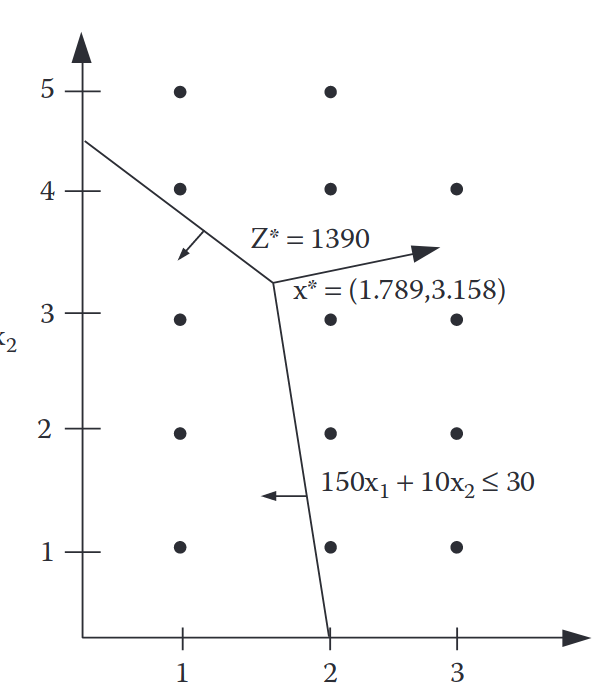
\includegraphics[width=0.4\linewidth]{../figures/IntegerProgramming.png}
    \end{center}
    Graphical representation of a typical 2 dimensional integer programming\cite{carter}.
  \end{frame}

\section{IP examples}

  \begin{frame}
    \frametitle{Integer problem examples}
  
    \begin{itemize}
      \item Capital budgeting: deciding between a collection of investiments
      \item Warehouse location: in modelling distribution systems, we should decide about tradeoffs between transportation costs and costs for operating distributions centers
      \item Scheduling: students-faculty-classrooms allocations, vehicle dispatching, etc (see next slide)
    \end{itemize}
  
  \end{frame}

\begin{frame}
  \frametitle{\href{https://fastercapital.com/content/Optimization--Solving-Complex-Problems-with-Zero-One-Integer-Programming.html}{Zero-One (0-1) scheduling problem}}

  {\bf Airline crew scheduling problem}: The airlines first design a flight schedule composed of a large number of {\em flight legs} (specific flight on a specific piece of equipment, such as a 747 from New York to Chicago departing at 6:27 a.m.). A flight crew is a complete set of people, including pilots, navigator, and flight attendants who are trained for a specific airplane. A work schedule or rotation is a collection of flight legs that are feasible for a flight crew, and that normally terminate at the point of origin. Variables $x_{ij}$ have value 1 if flight leg $i$ is assigned to crew $j$. All flight legs should be covered at minimum total cost. 
  \\[10pt]
  Also called a {\em set-partitioning problem}
  \begin{equation*}
    \begin{aligned}
      \text{minimize } \quad & \sum_{j=1}^{n} c_j x_j \\
      \text{subject to }\quad &
      \begin{array}{rcl}
        \sum_{j=1}^n a_{ij} x_j= 1&i=1,2,\ldots,m&  \\
        x_j = {0,1} &j=1,2,\ldots,n
      \end{array}
    \end{aligned}
  \end{equation*}

\end{frame}

\begin{frame}
  \frametitle{Travelling salesman problem}

  \begin{Exercise}
    Consider the travelling salesman problem. Starting from his home, a salesman wishes to visit each of $(n-1)$ other cities and return home at minimal cost. He must visit each city exactly once and the cost to travel from city $i$ to $j$ is $c_{ij}$. Let $x_{ij}$ be 1 or 0 depending on the fact that he goes or not from city $i$ to city $j$
    \begin{itemize}
      \item formulate the optimization problem
      \item how to avoid disjoint tours?
    \end{itemize}
  \end{Exercise}

\end{frame}


\begin{frame}{Applications of the Traveling Salesman Problem (TSP)}
  \begin{itemize}
      \item \textbf{Logistics and Supply Chain:} Delivery route optimization for couriers (e.g., FedEx, UPS), and minimizing travel distances for food delivery services (e.g., Glovo).
      \item \textbf{Manufacturing:} Efficient routing of robotic arms in assembly lines, and optimal sequencing of drilling or cutting operations in circuit board manufacturing.
      \item \textbf{Telecommunications:} Designing optimal fiber optic or cable routing networks, and planning routes for signal maintenance teams.
      \item \textbf{Travel and Tourism:} Planning shortest tour routes for sightseeing in cities, and organizing efficient itineraries for travel agencies.
      \item \textbf{Biology and Genetics:} DNA sequencing, where TSP helps align fragments of genetic material.
      \item \textbf{Other Examples:} School bus routing, and urban planning and traffic management.
  \end{itemize}
\end{frame}

\section{Solving integer problems}

\begin{frame}
  \frametitle{Solving Integer problems}

  Simplex is not useful to solve, in general, integer problems. Instead, many other techniques have been proposed:
  \begin{itemize}
    \item Enumeration techniques, including the branch-and-bound procedure;
    \item cutting plane techniques; and 
    \item group-theoretic techniques,
  \end{itemize}

  as well as several composite techniques
  

\end{frame}



  \begin{frame}
    \begin{center}
      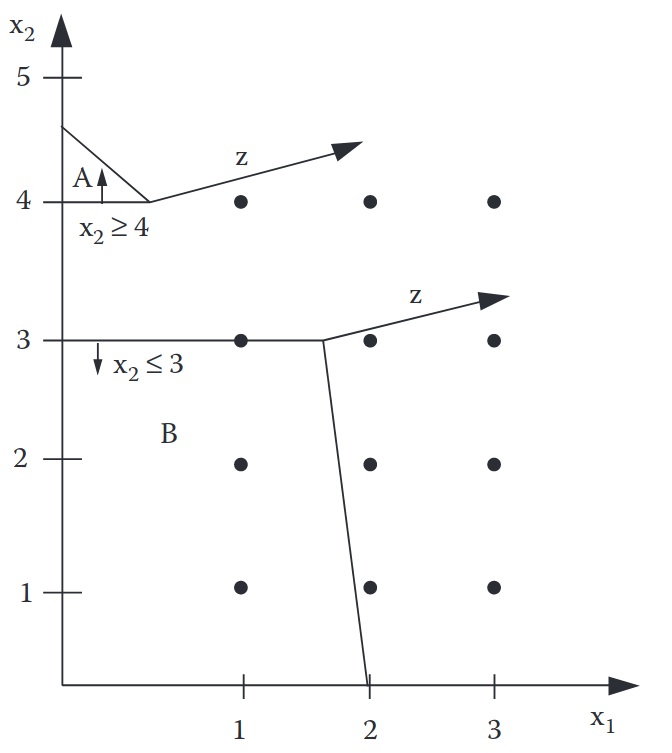
\includegraphics[width=0.4\linewidth]{../figures/BranchandBound.png}
    \end{center}
    Separation into two subproblems in the Branch-and-Bound method\cite{carter}.
  \end{frame}

\begin{frame}

  \begin{Exercise}
    Using the graphical representation and the branch-and-bound procedure, solve this integer program:
    \begin{equation*}
      \begin{aligned}
        \text{maximize } \quad & z=x_1+5x_2 \\
        \text{subject to }\quad &
        \begin{array}{rcl}
          -4x_1+3x_2\leq 6&&  \\
          3x_1+2x_2\leq 18&&  \\
          x_1,x_2 \geq 0 & \mathrm{and\,integer}
        \end{array}
      \end{aligned}
    \end{equation*}
  \end{Exercise}

\end{frame}


\section{References}
\begin{frame}{References}
    \footnotesize
    \begin{thebibliography}{99}
    \setbeamertemplate{bibliography item}[text]
      \begin{columns}[t]
        \begin{column}{.45\textwidth}
            \bibitem{carter} Michael W. Carter, Camille C. Price, and Ghaith Rabadi. Operations Research, 2nd Edition. CRC Press.
            \bibitem{harel} David Harel, with Yishai Feldman. Algorithmics: the spirit of computing, 3rd Edition. Addison-Wesley.
            \bibitem{rardin} Ronald L. Rardin. Optimization in Operations Research, 2nd Edition. Pearson.
            \bibitem{hefferon} J. Hefferon. \href{http://joshua.smcvt.edu/linearalgebra}{Linear algebra (4th Ed)}.
        \end{column}
        \begin{column}{.45\textwidth}
            \bibitem{riley} K.F. Riley, M.P. Hobson, S.J. Bence. Mathematical Methods for Physics and Engineering (2nd Ed). McGraw Hill.
            \bibitem{nocedal} J. Nocedal, S. J. Wright. Numerical Optimization (2nd Ed). Springer.
            \bibitem{beers} Kenneth J. Beers. Numerical methods for chemical engineering: applications in Matlab. Cambridge University Press.
            \bibitem{barber} D. Barber. Bayesian reasoning and machine learning. Cambridge University Press.
        \end{column}
      \end{columns}
    \end{thebibliography}
\end{frame}
%----------------------------------------------------------------------------------------

\end{document}
